\section{Microcontrollers}

Microcontrollers are specifically designed to perform targeted computational tasks. 
These devices incorporate small, integrated memory solutions.
\begin{figure}[H]
    \centering
    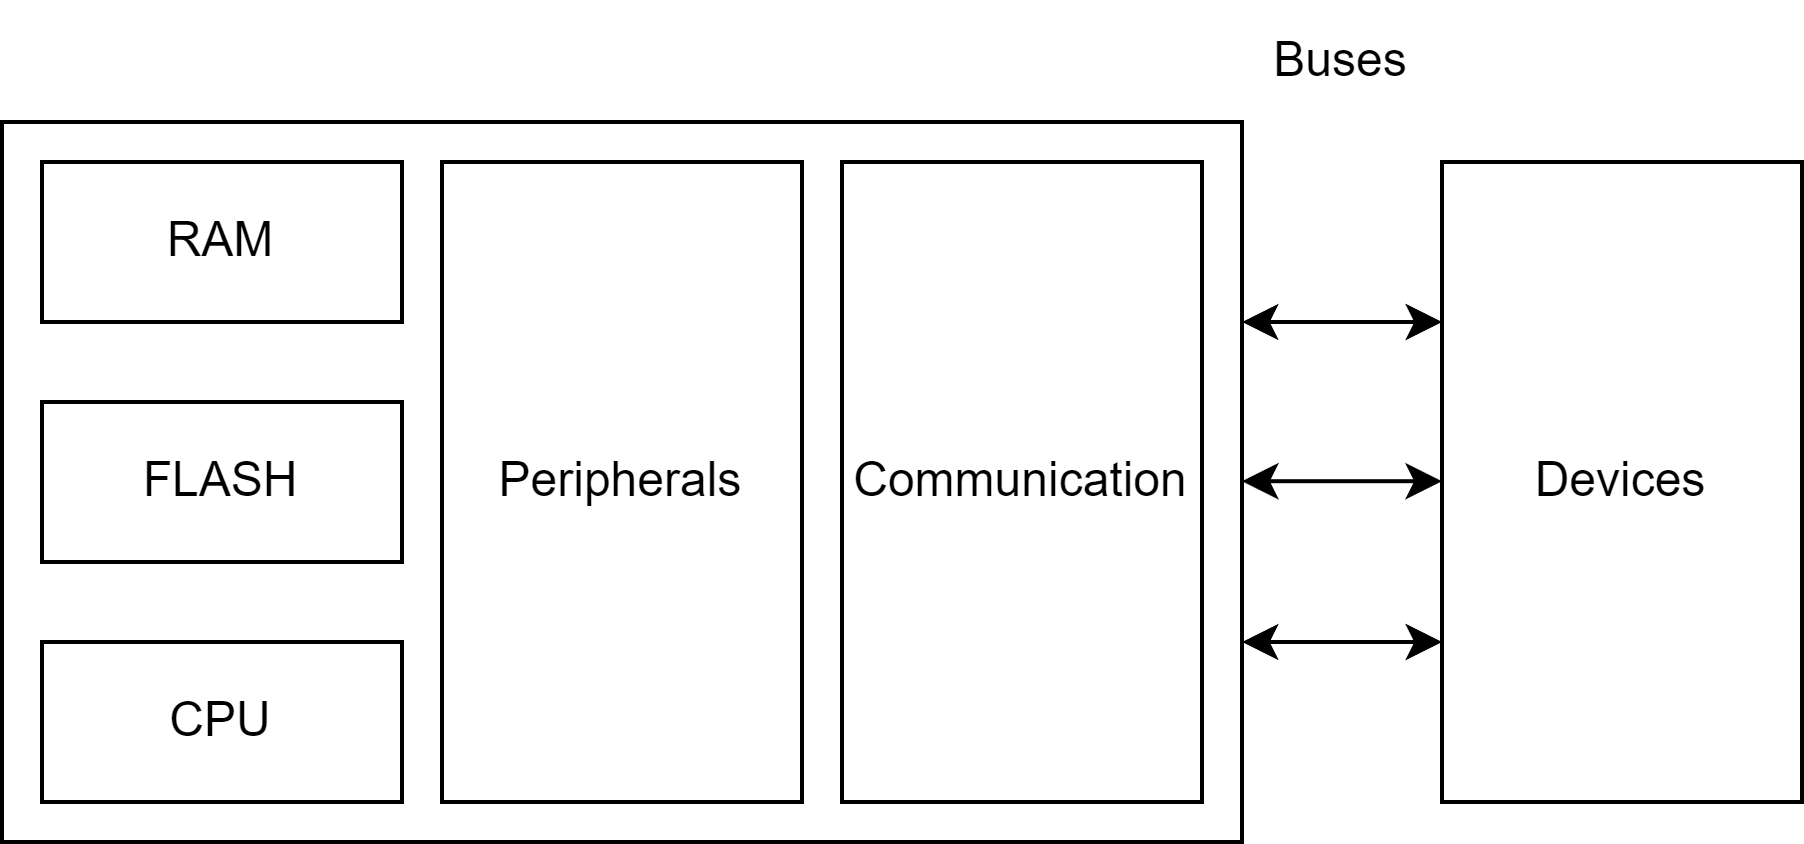
\includegraphics[width=0.75\linewidth]{images/miccon.png}
    \caption{Microcontroller architecture}
\end{figure}

\subsection{Subsystems}
The main subsystems in microcontrollers are: 
\begin{itemize}
    \item \textit{Clock}: fundamental component that synchronizes all subsystems (core, memories, and peripherals). 
        Usually, we have two types of clock: 
        \begin{itemize}
            \item \textit{Main clock}: drives core, memories, and peripherals (from 2 to 144 MHz). 
            \item \textit{Real Time Clock} (RTC): used for timekeeping (usually $\approx$ 32 Hz). 
                It serves two primary functions timekeeping and periodic alarm generation.
                It is designed for high accuracy over extended periods. 
                To achieve accurate timing, periodic resynchronization with external sources is necessary.
                
                RTC can be used to count periodically (timers) or check periodically some subsystems (watchdogs).
                Watchdogs are configured once during the boot process, it is set to trigger an interrupt or reset at a fixed time interval. 
                There are two primary modes of operation for watchdog timers: non-windowed (cleared before a specified time) and windowed (cleared within a specific time). 
        \end{itemize}
        The clock could be originated by internal oscillators (imprecise due to heat, djusted through a Digital Phase Locked Loop) or external oscillators (accurate, frequency adjusted with a DPLL or a crystal). 
        The main clock can be modulated by dedicated clock generation and distribution logic, which enables various clock feeds to supply different groups of elements (called domains). 
        Clock management consists in mantaining low drift, low temperature, and high accuracy. 
        To lower the power consumption techniques such as frequency scaling and clock gating are employed. 
    \item \textit{Memory}: usually, it is characterized by a single addressing space (with 16 or 32 bit addresses). 
        Various types of memory are mapped to different regions within this same addressing space, eliminating the need for a cache in many cases. 
        
        When the addreesing space is limited we may use banked memory (that composes a subset of the global memory). 
        Thus, in this case we have differences between local and global addresses. 

        In case of wide address we need some specialized registers that necessistates special memory to be handled. 
    \item \textit{General Purpose Input Output} (GPIO): GPIO pins are capable of serving multiple functions such as digital and analog input, and  analog input output. 
        Those pins are organized into groups known as ports. 
        To manage these functionalities effectively, several registers are utilized:
        \begin{itemize}
            \item \textit{Data Direction Register} (DDR): defines the direction of each pin.
            \item \textit{Port Data Register} (PDR): holds the data for the pin when it is used in digital mode.
            \item \textit{Port Pin State Register} (PPSR): checks the current state of the port pins (used for real-time monitoring of statuses).
            \item \textit{Edge Port Control Registers} (EPCR):configure pins for various detection modes (level detection and detection of rising or falling edges). 
                They also enable or disable interrupts related to specific pins and manage internal pull-up or pull-down resistors.
            \item \textit{Edge Port Status Register} (EPSR): maintains status flags associated with pins that have interrupt capabilities.
        \end{itemize}
    \item \textit{Analog comparators}: specialized differential amplifiers designed to compare two input voltages, saturating the output to either the supply voltage or ground. 
        Given two inputs voltages $A$ and $B$, and an ouptu $Y$, the behavior of the analog comparator is straightforward:
        \[Y=\begin{cases} 1 \qquad\text{if } A> B \\ 0 \qquad\textit{otherwise} \end{cases}\]
        This behaviour could be inverted through polarity selection. 

        Analog comparators can be used for various purposes: 
        \begin{itemize}
            \item \textit{Polling}: based on the output value, the software can perform slow operations.
            \item \textit{Interrupt}: the comparator's output is connected to an interrupt controller. 
                When a comparison event occurs, an interrupt service routine is executed. 
            \item \textit{Hardware}: the output of the comparator is fed directly to an output pin.
            \item \textit{Hardware count or capture}: the output is connected to a control input of a timer. 
                In count mode, every change in the output generates a front that is counted
                In capture mode, the system measures the time interval between two fronts. 
        \end{itemize}
    \item \textit{Analog to digital converter} (ADC): encodes an input voltage signal into a numeric value. 
        The steps performed by the ADC are:
        \begin{enumerate}
            \item \textit{Sampling}: the input signal is observed based on a periodic time base. 
            \item \textit{Quantization}: rounds the real valued physical quantity of the input signal to fixed discrete intervals determined by the power supply voltage. 
                This process converts the continuous signal into a finite set of values.
        \end{enumerate}
        Accurate timing is essential for the proper functioning of an ADC (with the main clock). 

        The perfromance is dependent on the stability of the power supply. 
        To mitigate this issue, ratiometric measurement techniques are employed, which require a fixed absolute voltage reference to maintain accurate readings.

        One important function of the ADC is input multiplexing (multiple analog inputs are connected and converted cyclically). 
    \item \textit{Communication}: there are multiple buses available: 
        \begin{itemize}
            \item \textit{Serial Peripheral Interface} (SPI): synchronous communication protocol used to transfer data between a single master and multiple slave devices.
                The communication is synchronized through a clock signal generated by the master, allowing high-speed data transfer rates. 
                SPI uses three primary lines: MISO (Master In, Slave Out), MOSI (Master Out, Slave In), and SCK (Serial Clock). 
                A separate line, SS (Slave Select), is used to choose which slave device the master communicates with.

                In multi-slave configurations, connecting $N$ slave devices requires $3 + N$ lines, as each device is selected by its dedicated SS line. 
                One of the strengths of SPI is that devices can operate at different speeds, making it adaptable for various systems.

                During transmission, the master asserts the SS line to select the target slave, generates clock pulses, and sends data to the slave on the MOSI line. 
                In reception, the master selects the slave, sends clock pulses, and transmits dummy data on the MOSI line while receiving actual data from the slave on the MISO line.

                In full-duplex data transfers, SPI allows the master to send data to the slave on MOSI while simultaneously receiving data from the slave on MISO. 
                To account for delays between read and write operations, dummy bytes can be added at the beginning or end of the data frames.
            \item \textit{Universal Asynchronous Receiver Transmitter} (UART): point-to-point asynchronous communication protocol with medium data transfer rates that involves a transmitter (Tx) and a receiver (Rx).
                Hardware flow control can be implemented in UART to allow devices to negotiate when to start or stop the transmission of data.
                The Ready To Send (RTS) signal indicates that the transmitter is ready to send data, while the Clear To Send (CTS) signal is used by the receiver to inform the transmitter when it is ready to receive data.

                In UART, data transmission is organized into frames. 
                A typical frame consists of a start bit, followed by 7 or 8 data bits, an optional parity bit (used for error detection), and one or two stop bits.

                In operation, the transmitter sends bits over the Tx line, while the receiver reads them from the Rx line. 
                If hardware flow control is used, the transmitter first asserts the RTS signal, indicating it is ready to send.
                When the receiver is ready, it asserts the CTS signal, allowing the transmission to proceed. 
                The transmitter then sends bits over the Ex line, and the receiver reads them over the Rx line. 
                If the receiver needs the transmitter to pause, it de-asserts the CTS signal, causing the transmitter to suspend sending until the receiver re-asserts CTS.
            \item \textit{Inter Integrated Circuit} (I$^2$C): synchronous communication protocol designed to allow communication between multiple devices, including multiple masters and slaves.
                The protocol uses two lines: a bidirectional data line (SDA) and a clock line (SCL), both shared by all devices on the bus.

                I$^2$C supports multiple slaves without needing additional lines for each slave, as required in SPI. 
                It has lower data rates compared to SPI
        
                In a typical I$^2$C configurations, a single master communicates with multiple slave devices. 
                The master initiates all data transfers and generates the clock signal. 
                Both the master and the slaves can control the data line depending on whether the operation is a read or write.

                In a write operation, the master generates a start condition and sets up to write by sending the slave address with the read and write bit set to 0. 
                The master then sends the data chunks, with the slave acknowledging each chunk, and the master finally ends the operation by generating a stop condition.

                In a read operation, the master begins similarly by generating a start condition and setting up to read, sending the slave address with the read and write bit set to 1. 
                The slave acknowledges and then sends data chunks, which the master acknowledges. 
                Once the read is complete, the slave does not acknowledge, and the master generates a stop condition.

                I$^2$C also supports combined transfer operations, where a write and a read occur in a single transaction. 
                In this case, after the initial write operation, the master generates a repeated start condition and then initiates a read operation. 
                Data is exchanged in the same way, with the master acknowledging until the transfer is complete. 
                After receiving all the data, the master sends a stop condition to terminate the communication.
        \end{itemize}
\end{itemize}